\chapter{基于LTL的表示与决策方法}\label{ltl}
本章提出一种基于LTL的智能体目标和norm的表示方法,并将其与\SA 算法结合,提出一种同时支持实现型目标、维持型目标以及norm的意图调度算法\SAT。本章实验部分对\SAT 的性能表现在不同的资源储备量下进行了分析,并与Duff等人提出的PMG\cite{DBLP:conf/atal/DuffHT06}算法和Meneguzzi等人提出的v-BDI算法\cite{DBLP:journals/eaai/MeneguzziROVL15}进行了比较,实验结果表明\SAT 的性能表现相对PMG和v-BDI有显著优势\footnote{在前两章中,本文分别将\SAM 与PMG进行对比,将\SAN 与v-BDI进行对比。}。
\section{多类型的目标与norm}
在许多社会仿真场景中,目标可能有丰富的类型,例如需要智能体在一段时间内保持某一特定状态的维持型目标,或是在某些特定情况下,只有在满足某些特定条件时才最求的条件目标。此外,智能体的行为可能受到norm的约束,智能体需要在决策时加入对norm的考虑,以避免违反norm,或者选择性地违反norm以实现更重要的目标。本文第\ref{mg}章研究了了如何同时对实现型目标和维持型目标进行意图调度,并提出了\SAM 算法;第\ref{norm}章研究了了如何在norm约束下进行意图调度,并提出了\SAN 算法。本章考虑更为实际的社会仿真模拟场景:在本章中,各种类型的目标与norm统一以线性时序逻辑(Linear Temporal Logic, LTL)的形式表示,而智能体需要对LTL表示的目标或norm进行意图调度。

Dastani等人\cite{DBLP:conf/atal/DastaniRW11}提出了一种基于LTL表示各种类型目标(如实现型目标、维持型目标、行动目标等)的框架。在其框架中一个维持型目标被表示为$\alpha \cup \tau$,其中$\alpha$为智能体需要维持的条件,$\cup$表示“直到”,而$\tau$表示终止条件。因此$\alpha \cup \tau$表示维持$\alpha$,直到$\tau$被满足。LTL的表示能力是通用且强大的,足以表示各种类型的目标并拓展现有目标类型。为了实现这些LTL形式的目标Dastani等人也在其研究中提出一种转换方法,能够将LTL公式转变为一般智能体编程语言所支持的普通实现型目标和维持型目标。其LTL目标的转化规则以条件-动作对(Condition-Action Pairs)来表示。其描述了在某个特定环境状态下的目标状态转变(由LTL目标转化为基本目标)。Dastani等人\cite{DBLP:conf/atal/DastaniRW11}描述了两种类型的条件-动作对:通用性的以及领域专用的条件-动作对。通用性的条件动作对适用于该框架给定的目标形式,而领域专用的条件-动作对则是为特定领域设计的针对特殊表示形式目标的转换方法,目的是提升智能体的适用范围。然而,该框架并没有提供一个一般性的意图调度算法,某些特殊形式的目标仍然需要用户自定义条件-动作对,虽然有一点的拓展性,但加重了用户的负担;此外,该框架也没有考虑到社会仿真场景下的norm,这导致其不适用于norm约束场景。

Gutierrez等人\cite{DBLP:conf/time/0001KPW22}提出了用于向智能体发出指令的语义模型。该研究以LTL公式的形式表示指令,而智能体则必须以确保LTL公式得到满足的方式行动。此外,该研究假定智能体有一定的后台安全需求(同样以LTL形式表示)需要智能体保护(类似于维持型目标)。该研究对LTL满足(如何行动以满足LTL)与LTL生成(如何根据需求生成LTL)的时间与空间复杂度进行了细致分析。然而,正如其作者所提到,将该语义模型应用于实际的好处仍然未知,因为其并没有被实际应用,无相关实验分析,而仅为一种可能有价值的理论。

Krzisch等人\cite{Krzisch2016}基于经典的规划问题对norm系统进行建模。其考虑了两种norm形式化的方法:一种是仅仅考虑某些场景下的动作(允许或是禁止执行某些动作);另一种则是LTL约束下的一系列状态转移。该研究提出了相应算法以应对norm的约束,然而其算法并没有考虑到多种类型的目标,并且也忽略了多个并发意图下的意图进展问题。

Paxton等人\cite{DBLP:journals/corr/PaxtonRHK17}提出了一种基于深度强化学习的方法以解决复杂动态环境中的规划问题。而该问题被规范表示为一组LTL公式。该方法将MCTS与基于LTL规范训练的人工神经网络结合。该研究在一个仿真自动驾驶场景对人工神经网络的学习能力进行了评估。然而,其在模拟场景下的学习效果并不如预期,并且智能体偶尔会出现奇怪行为。另外,该研究的重点也与对智能体目标、norm的表示关联不大。


\section{使用LTL表示目标与norm}
使用LTL表示目标和norm的优势在于智能体可以在更高的抽象层次处理目标和norm的特性,并且更意图拓展目标和norm的类型。LTL是一种模态时序逻辑方式方式。其由一组有限的命题变量、逻辑运算符(如$\lnot, \lor$)以及时间运算符组成。本文考虑以下时间运算符:
\begin{itemize}
    \item $\square$ 表示是“一直”
    \item $\diamond$ 表示“最终”
    \item and $U$ 表示是“直到”
\end{itemize}
由于在本章中目标和norm基于LTL表示,而LTL编码了状态随时间变化的轨迹,所以本节内容首先对环境及其状态转换进行定义。在此基础上,再给出基于实现型目标、维持型目标以及norm的LTL表达形式(这些目标和norm的表示只是实例,正如\cite{DBLP:conf/atal/DastaniRW11},LTL支持其他更加丰富的目标和norm类型)。

\subsection{环境及其状态转移的表示}
Gutierrez等人\cite{DBLP:conf/time/0001KPW22}描述了一种表示环境及其状态变化的方法。本文基于其方法,对环境以如下方式表示。

本文假设智能体在一个特定的环境中执行,该环境可以处于包含所有可能环境状态集合中的任意一个状态。每个状态都由一组环境变量$V$的确定赋值决定。智能体有一动作集合$\mathcal{A}$,$\mathcal{A}$中的动作可在其前置条件满足时被执行。环境状态从$s_0$开始执行,在一个状态下执行某个动作的结果是将当前环境状态$s$转化为下一个环境状态$s^\prime$。该转变规则由一个转变函数所决定:$\mathcal{T} (s, a) = s^\prime$(为了简单起见,本文假设转变函数为确定型)。在此,本文仅考虑环境状态及其转变,智能体本身的内部状态(如信念、意图等)不在考虑范围内;对于智能体而言,仅仅考虑到能够直接影响到环境状态改变的动作。

形式上,环境由一五元组$E=<\mathcal{S}, V, \mathcal{A},\mathcal{T}, s_0>$所表示,其中:
\begin{itemize}
    \item $\mathcal{S}$为包含所有可能环境状态的非空有限状态集合。
    \item $V$为表示所有环境变量的非空有限集合。
    \item $\mathcal{A}$为智能体可执行的动作集合。
    \item $\mathcal{T}: \mathcal{S} \times \mathcal{A} \rightarrow 2^{\mathcal{S}}$为状态转变函数。
    \item $s_0 \in \mathcal{S}$表示初始环境状态。
\end{itemize}
智能体遵循其运行策略执行动作,直到没有可执行的操作或所有目标都被实现。基于此通识,智能体在环境中执行动作的过程会产生出环境状态与动作的交错序列,该序列被称为\emph{游程}:
\begin{equation}
\rho=s_0 \xrightarrow{\text{$a_0$}} s_1 \xrightarrow{\text{$a_1$}} s_2 \xrightarrow{\text{$a_2$}} \cdots \xrightarrow{\text{$a_{n-1}$}} s_n
\end{equation}
其中$\rho$表示一次游程,本文使用$si(\rho, u)$来索引第$u$个状态,使用$ai(\rho, u)$来索引$\rho$中的第$u$个动作(其中$u$为一个自然数)。本文假设一个游程是有限的,即有一个表示$\rho$结束的最终状态$s_n$。

\subsection{目标、norm的表示}
本文第\ref{mg}章对实现型目标和维持型目标进行了定义,第\ref{norm}章对norm进行了定义,然而并没有对其形式进行统一。
本节正式基于LTL对实现型目标、维持型目标以及norm进行定义。通过这样做,在考虑新的形式的目标和norm时,可以免去对智能体程序的大量修改。智能体仅需要处理新添加的LTL公式即可。此外,这更加便于开发处理丰富类型目标和norm的意图调度算法。

\paragraph{实现型目标}
实现型目标表示了智能体想要达到的环境状态,实现型目标的定义如下:
$$<G_a, C_g, Pls, Val>$$
其中$G_a$为该目标的名称, $C_g$为目标条件,表示为$\diamond s_g$;$s_g$为一组非时序的语句,表示智能体想要达到的环境状态,这意味着智能体需要在某个时间节点实现$s_g$;$Pls$为一组可用于实现目标的计划,$Val$为以正数,表示该目标的价值。

\paragraph{维持型目标}
维持型目标表示智能体在某些情况下需要维持的环境状态,其定义如下:
$$<G_m, C_m, Pls>$$
其中$G_m$为该维持型目标的名称, $C_m$为维持型条件,表示为$\square (\tau \rightarrow (s_m \mathsf{U} \mu))$,其中$s_m$和$\tau$一组语句。该LTL公式的含义是,需要在$\tau$被满足之后且$\mu$被满足之前保持$C_m$状态。当$C_m$不满足时,可执行$Pls$中的计划以修复维持条件。

\paragraph{norm}
norm定义了智能体在某些特定情况下可以做什么、需要做什么以及禁止做什么,其定义如下:
$$<N_n, C_n, Val>$$
其中$N_n$为该norm的名称, $C_n$为触发条件,表示为$\square (\tau \rightarrow ( \diamond done(a) \mathsf{U} \mu))$,其中$\tau$为实际触发条件,$\mu$为失效条件。 $done(a)$ 表示动作$a$已被执行的事实。因此,该触发条件意味着在满足$\tau$之后且$\mu$被满足之前执行动作$a$会触发norm,并受到价值为$Val$的后果。$Val$可以为正数、0或负数,分别代表义务norm(智能体需要执行$a$),许可norm(智能体可以执行$a$),以及禁令norm(智能体禁止执行$a$)。
与第\ref{norm}章相同,本章假设norm所谓软约束实现,因此不限制智能体的灵活性,智能体可以根据价值$Val$以及自身的执行策略选择遵守或违反norm。
\subsection{基于目标计划树模型的问题定义}
本节对IPP的原始定义进行拓展,加入对用LTL表示的目标与norm的考虑。具体地,基于目标计划树模型,LTL形式下的意图进展问题可被定义为:给定一组表示智能体意图的目标计划树$\{t_1, \dots, t_n\}$,一组智能体需要满足的LTL公式以及一组表示智能体当前环境状态的条件变量$env$,在每一个执行周期中返回一个目标计划树$t_i$中的下一个执行步骤使得智能体获得的总价值最高。
\section{\SAT 意图调度算法}
本章介绍同时考虑实现型与维持型目标的意图调度算法\SAT 。\SAT 在\SA(已在第\ref{SA}章节中介绍)的基础上进行拓展,加入对LTL公式的处理。

在\SA 的模拟阶段,每次模拟运行结束时返回实现目标获得的总价值。由于目标条件被定义为一组语句,检查目标是完成的过程相对简单:如果目标条件得到满足,则其相应的目标被视为完成。然而,当考虑LTL形式表示的目标和norm时,需要额外的算法检查LTL公式是否得到满足。

为了支持LTL公式的意图调度算法,本研究首先提出一种检查一游程是否满足给定LTL公式的算法。在此基础之上,再对\SA 算法的扩展和模拟阶段进行修改。

\subsection{LTL检查器}
本节介绍一个用于检查LTL的基本框架,其可以检查一游程$\rho$是否满足一给定的LTL公式。
LTL检查器的基本步骤如图\ref{fig:translator}所示。检查器首先使用LTL解析器和转换器将LTL公式转换为与其等效的状态机,然后由状态机读取游程序列并检查是否满足。
LTL解析器和转换器已在\cite{DBLP:books/daglib/0020982,DBLP:journals/jlap/HuangC22}中实现,在\cite{DBLP:books/daglib/0020982}中,状态机用于检查无穷状态转移序列,而在\cite{DBLP:journals/jlap/HuangC22}中,状态机用于检查有限状态转移序列。

\begin{figure*}[htb]
\centering
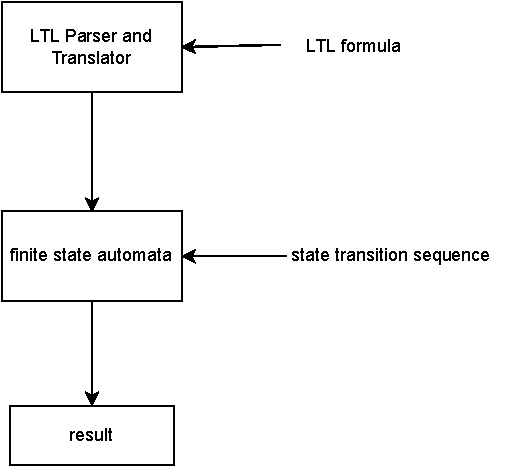
\includegraphics[width=0.9\textwidth]{./figs/translator}
\caption{LTL Checker}
\label{fig:translator}
\end{figure*}

以下为基于该框架的LTL检查算法:
\begin{algorithm} % This algorithm can also be used
\caption{LTL Checker}\label{checker}
\begin{algorithmic}[1]
\STATE input:$(\rho, o)$
\STATE $l \gets getLTL(o)$
\STATE $\alpha \gets transform(l)$ \COMMENT{transform LTL to automaton}
\FOR{$i \leftarrow 0, len(\rho)-1$}
  \STATE $s \gets si(\rho, i)$
  \IF {$\alpha.isTransitable(s)$}
    \STATE $\alpha.transit(s)$
    \ELSE
    \STATE $trigger(o)$
  \ENDIF
\ENDFOR
\IF {$o$ is an achievement goal and $\alpha$ is in final state}
  \STATE $o.achieved()$
\ENDIF
\end{algorithmic}
\end{algorithm}
该检查器的输入参数有两个:游程$\rho$和一个LTL对象$o$。
%
% @TODO: line number ref.
检查器首先得到LTL公式并将其转化为状态机。然后$\rho$中的每个状态都由状态机迭代处理并根据每个环境状态进行状态机的状态转移\footnote{注意,环境状态与状态机中的状态是两个不同的概念。};如果状态机可在当前环境状态下进行转换,则应用该转换。否则,状态机不接收当前环境状态,其相应LTL对象被触发。对于维持型目标,出发意味着维持条件不满足,智能体此时应执行相关修复计划;对于norm,触发意味着norm被触发且智能体收到相应的价值;最后,如果该LTL公式对应一个实现型目标,并且状态机处于其最终状态(Final State),那么该目标被视为已实现。

算法\ref{trigger}所示的触发函数用于对触发LTL对象的相应操作。
\begin{algorithm} % This algorithm can also be used
\caption{trigger function}\label{trigger}
\begin{algorithmic}[1]
\STATE input:$(o)$

\IF {$o$ is a maintenance goal and no recover plan is adopted}
\STATE adopt a recover plan
\ELSE
\IF {$o$ is a norm}
\STATE receive value $o.Val$
\ENDIF
\ENDIF

\end{algorithmic}
\end{algorithm}

在描述对\SA 法的修改之前,本节首先描述智能体的初始设定以及骑在执行期间的内部状态转换规则:假设智能体在开始执行时被分配了一组需要满足的LTL公式,在正式执行之前,智能体首先将每个LTL公式转化为状态机(状态机为智能体内部状态的一部分);在智能体执行过程中,每次更新智能体信念集合时,所有状态机都会根据智能体当前对环境的认知进行状态转移;如果在当前认知下,状态机中可由可应用的状态转移规则,则按照算法\ref{checker}所述触发其相关操作。

\subsection{对\SA 法的修改}
为了支持LTL表示形式下的意图调度,\SAT 修改了\SA 算法中的扩展与模拟阶段,具体修改如下:
\paragraph{对扩展阶段的修改}
% Reactive
在扩展阶段,\SAT 首先检查某个选中的叶子节点$n_s$状态下每一个可执行动作$a_i$,若$a_i$所引发的(状态机的)状态转移不会使得智能体获得负收益,则直接生成一个新的节点对应于执行$a_i$的结果,并作为$N_s$的一个孩子节点。若$a_i$会引发负收益,则首先进行如下检查:检查$a_i$所对应的状态机$m_i$,若$m_i$可获得的最终的价值$V_i$大于当前执行$m_i$相关动作所受到的总惩罚值$P_i$(包括执行$a_i$的惩罚值),则生成一个新节点对应于执行$a_i$的结果。相反,若$m_i$可获得的最终价值$V_i$小于当前执行$m_i$相关动作所受到的总惩罚值$P_i$,则不生成新的节点。
%
当所有可执行动作$a_i$都会造成$P_i > V_i$时,则不会有新的节点生成。该情况下智能体会暂停其执行。
%
在\SAT 中,每个节点记录的信息除智能体意图、环境状态外,还记录了执行过程中所收到的总价值(收益值以及惩罚值)和每个状态机单独得到的价值。

\paragraph{对模拟阶段的修改}
在模拟阶段,\SAT 和\SA 一样,随机选择实现目标过程中可执行的动作执行。当某个可执行动作$a_i$造成状态机的状态转移并获得负收益时时,进行如下检查:检查$a_i$对应的状态机$m_i$,若可获得的最终的价值$V_i$大于当前执行$m_i$相关动作所受到的总惩罚值$P_i$(包括执行$a_i$的惩罚值),则禁止该动作的执行。相反,若$m_i$可获得的最终价值$V_i$小于当前执行$m_i$相关动作所受到的总惩罚值$P_i$,则直接执行。

当以下三个条件中的任意一个满足时,模拟阶段即停止:
\begin{enumerate}
  \item 所有状态机都处于最终状态。
  \item 并非所有状态机都处于最终状态,但是智能体无法执行相关动作将其带入最终状态。
  \item 所有的可执行动作$a_i$都会导致$m_i$可获得的最终价值$V_i$小于当前执行$m_i$相关动作所受到的总惩罚值$P_i$。
\end{enumerate}

\section{实验}
本章的实验场景与上一章类似,基于火星探测器的模拟场景(见图\ref{fig:marsrover})。不同的是同时考虑到了维持型目标和norm的情况。维持型目标与norm的相关场景设定与第\ref{mg}和第\ref{norm}相同,在此不再赘述。

% measring the agent performance
本实验根据三个指标对智能体的性能进行评估:完成目标的数量、电池消耗量以及总惩罚值。具体地,本实验根据评估函数$\frac{\#goals}{batteryConsumption} - penaltyValue$对智能体的性能进行评估,其中$\#goals$为实现目标的数量,$batteryConsumption$为电池消耗量,$penaltyValue$为因违反norm而受到的总惩罚值。该价值函数决定了智能体的综合性能表现。

本文将\SAN 与Duff等人\cite{DBLP:conf/atal/DuffHT06}提出的PMG(本章对RMG也进行了实验,其作为基准以衡量其他方法的性能)和Meneguzzi等人\cite{DBLP:journals/eaai/MeneguzziROVL15}提出的v-BDI进行比较。PMG和v-BDI算法分别在第\ref{mg}章和第\ref{norm}章有所解释,在此不再赘述。

在接下来的实验中,v-BDI的价值函数被设定为$\frac{\#goals}{batteryConsumption} - penaltyValue$。\SAN 算法设定为执行100次迭代($\alpha = 100$),每次迭代执行10次的模拟($\beta = 10$)。\SAN 的价值函数与v-BDI相同,设定为$\frac{\#goals}{batteryConsumption} - penaltyValue$。

\subsection{低电池容量实验}
以下实验中考虑智能体在低电池容量下设定的性能表现。在低电池容量设定下,智能体的电池容量被设定为40。具体实验结果如图\ref{}所示。

\paragraph{惩罚值分析}
如图所示,随着norm数量的增加,所有智能体受到的惩罚值也相应增加。RMG受到的惩罚值最大。其原因有三部分:
\begin{enumerate}
  \item RMG缺乏对norm的处理能力,所有违反norm的行为都被RMG所忽略;
  \item 其次,由于其意图调度策略的设定(FIFO规则),RMG没有考虑到多个意图间的交互,使得其在地图中的移动距离更长,这可能导致更多的norm违反情况发生;
  \item 最后,RMG以被动方式处理维持型目标,这也会导致其在地图中的移动距离更长。
\end{enumerate}
与NMG相比,PMG具有更好的性能表现,这是由于其主动性的应对维持目标策略:若实现下一个目标会破坏维持条件,智能体将首先返回基地充电再考虑实现目标。这种策略节省了很多执行步骤,从而减少了执行过程中违反norm的次数。v-BDI比NMG有更好的性能表现,因为其可以在计划选择阶段考虑避免对norm的违反,减少了norm的违反次数。
\paragraph{电量消耗分析}
虽然所有方法的电量消耗都随着目标数量的增加而增加,但是RMG和PMG的电量消耗并不会随着norm数量的增加而改变(当目标数量相同情况下)。这是因为norm并不会改变RMG和PMG实现目标的顺序和方式。尽管v-BDI在电量消耗方面与RMG有着几乎相同的性能表现,但是随着norm数量的增加,其电量消耗有一定微小变化。这是因为norm确实会影响其计划选择,这可能会影响智能体是否会意外实现其他目标,而意外实现其他目标最终会有节省电量的效果,导致与RMG有微小差异。从该图中可得到的一个重要信息是当norm数量增加时,MCTS消耗的电量有所增加。这是由于其效用函数的设置$\frac{\#goals}{batteryConsumption} - penaltyValue$,当norm的数量较多时,MCTS讲牺牲其利用多意图间协同效应的能力,以更好的避免违反norm。最后,相比于其他方法,MCTS仍然有着最优秀的性能表现。
\paragraph{总价值分析}
随着norm数量的增加,所有方法的总价值都相应降低。MCTS的性能明显优于其他方法。在norm的数量为10的情况下,当目标数量增加时,MCTS的性能只有略微下降。这是因为由于目标数量的增加,MCTS可以更好地利用多意图间的协同效应,因此,协同效应带来的优势克服了违反norm次数增加造成的危害,从而获得较高的总价值。然而,正如图中所示,当norm的数量较多时,违反norm的危害难以得到补偿。

\subsection{高电池容量实验}
以下实验中考虑智能体在高电池容量下设定的性能表现。在高电池容量设定下,智能体的电池容量被设定为120。具体实验结果如图\ref{}所示。

在高电池容量设定下,这四种方法的性能变化趋势与低电池容量实验相似。明显不同之处在于,高电池容量下各个方法的性能表现相较于低电池容量都有所增加。
\paragraph{惩罚值分析}
在惩罚值方面,RMG和PMG之间的差异比低电池容量下小很多。这是因为高电池容量下智能体有相对充足的电量一次执行多个任务,维持型目标被触发的可能性和次数降低,这造成主动和被动的维持型目标直接差异无法很好得到体现。然而v-BDI受益于其考虑norm的计划选择策略,其性能相比于RMG和PMG仍有较为明显的优势。最后,正如所预料的,MCTS拥有最好的性能表现。
\paragraph{电量消耗分析}
RMG、PMG和v-BDI在电量消耗方面具有几乎相同的性能,这同样也是因为在高电池容量下智能体很少触发维持型目标,使得这些方法最终的行为表现很类似,消耗的电量非常相近。
\paragraph{总价值分析}
RMG和PMG在总价值方面同样也具有几乎相同的性能表现。然而尽管与RMG和PMG相比,v-BDI在消耗电量方面并无优势,但其总价值却比RMG和PMG高很多。这是因为与RMG和PMG相比,v-BDI受到的惩罚值更低,导致最终的总价值更高。最后,由于同时考虑维持型目标、norm以及利用多意图间协同效应的能力,MCTS的性能表现相较于其他方法有着显著优势。

\section{本章总结}
本章提出了一种基于MCTS的意图调度算法\SAT 。\SAT 可以在norm约束下同时对智能体的实现型目标和维持型目标进行意图调度。另外,基于火星探测器的模拟场景,本章在迪电池容量以及高电池容量场景下对\SAT 的性能进行了分析。实验结果表明\SAT 与其他方法(PMG和v-BDI)相比有着显著的性能优势。
